
\chapter*{Lecture 34}

\begin{recall}{}{}
\begin{itemize}
\item -
\end{itemize}
\end{recall}




\subsection{Further convolution example}
\begin{exmp}{}
Let 
\begin{equation}
H(s)=\frac{1}{s^2(s-a)}
\end{equation}
find $h(t)$.

\textbf{Solution:}
From the table, we know that :
\begin{equation*}
\Lapl^{-1}\left(\frac{1}{s^2}\right)= t \qquad \text{and} \qquad \Lapl^{-1}\left(\frac{1}{s-a}\right)= e^{at} 
\end{equation*}
Therefore, we can use the convolution theorem :
\begin{equation*}
h(t)=t * e^{at}=\int^t_0\tau e^{a(t-\tau)}d\tau = e^{at} \int^t_0\tau e^{-a\tau}d\tau
\end{equation*}
We can integrate by parts to find:
\begin{equation*}
h(t)=\frac{1}{a^2}\left(e^{at}-at-1\right)
\end{equation*}


\end{exmp}


\subsection{LT of discontinuous functions}
(where $H$ is a Heaviside function)
\begin{align*}
\Lapl[H(t-a)]&=\int^\infty_0 e^{-st}H(t-a) dt\\
&=\int^a_0 e^{-st}\underbrace{H(t-a)}_{=0}dt+\int^\infty_a e^{-st}\underbrace{H(t-a)}_{=1}dt\\
&=\int^\infty_a e^{-st}dt=\left.-\frac{1}{s}e^{-st}\right|^\infty_a
\end{align*}
We find:
\begin{align*}
\Lapl[H(t-a)]&=-\frac{1}{s}\left[0-e^{-as}\right]=\frac{1}{s}e^{-as} \qquad \text{for } s>0
\end{align*}

This can be extended to slightly more complex problems:
\begin{align*}
\Lapl[H(t-a)f(t-a)]&=e^{-as}\Lapl\left[f(t)\right]\\
\Lapl[H(t-a)f(t)]&=e^{-as}\Lapl\left[f(t+a)\right]\\
\end{align*}

\begin{exmp}{}
\begin{align*}
\Lapl\left[t^2 H(t-1)\right]=e^{-s}\Lapl\left[f(t+1)\right]&=e^{-s}\Lapl\left[(t+1)^2\right]\\
&=e^{-s} \Lapl[t^2+2t+1]=e^{-s}\left(\frac{2}{s^3}+\frac{2}{s^2}+\frac{1}{s}\right)
\end{align*}
\end{exmp}

\section{Application of LT}
\begin{exmp}{}
Consider the following problem shown in figure \ref{fig:prob}. The tank initiially holds 500 L of a brine solution with a salt concentration of 0.2 kg/L. For the first 10 min or operation, valve A is open, adding 12L/min of brine containing 0.4kg/L salt concentration. After 10 min, valve B is switched on, addiing 0.6 kg/L concentration at 12L/min. The exit valve C removes 12L/min. Find the concentration of salt in the tank as a function of time.\\

\begin{figure}
\centering
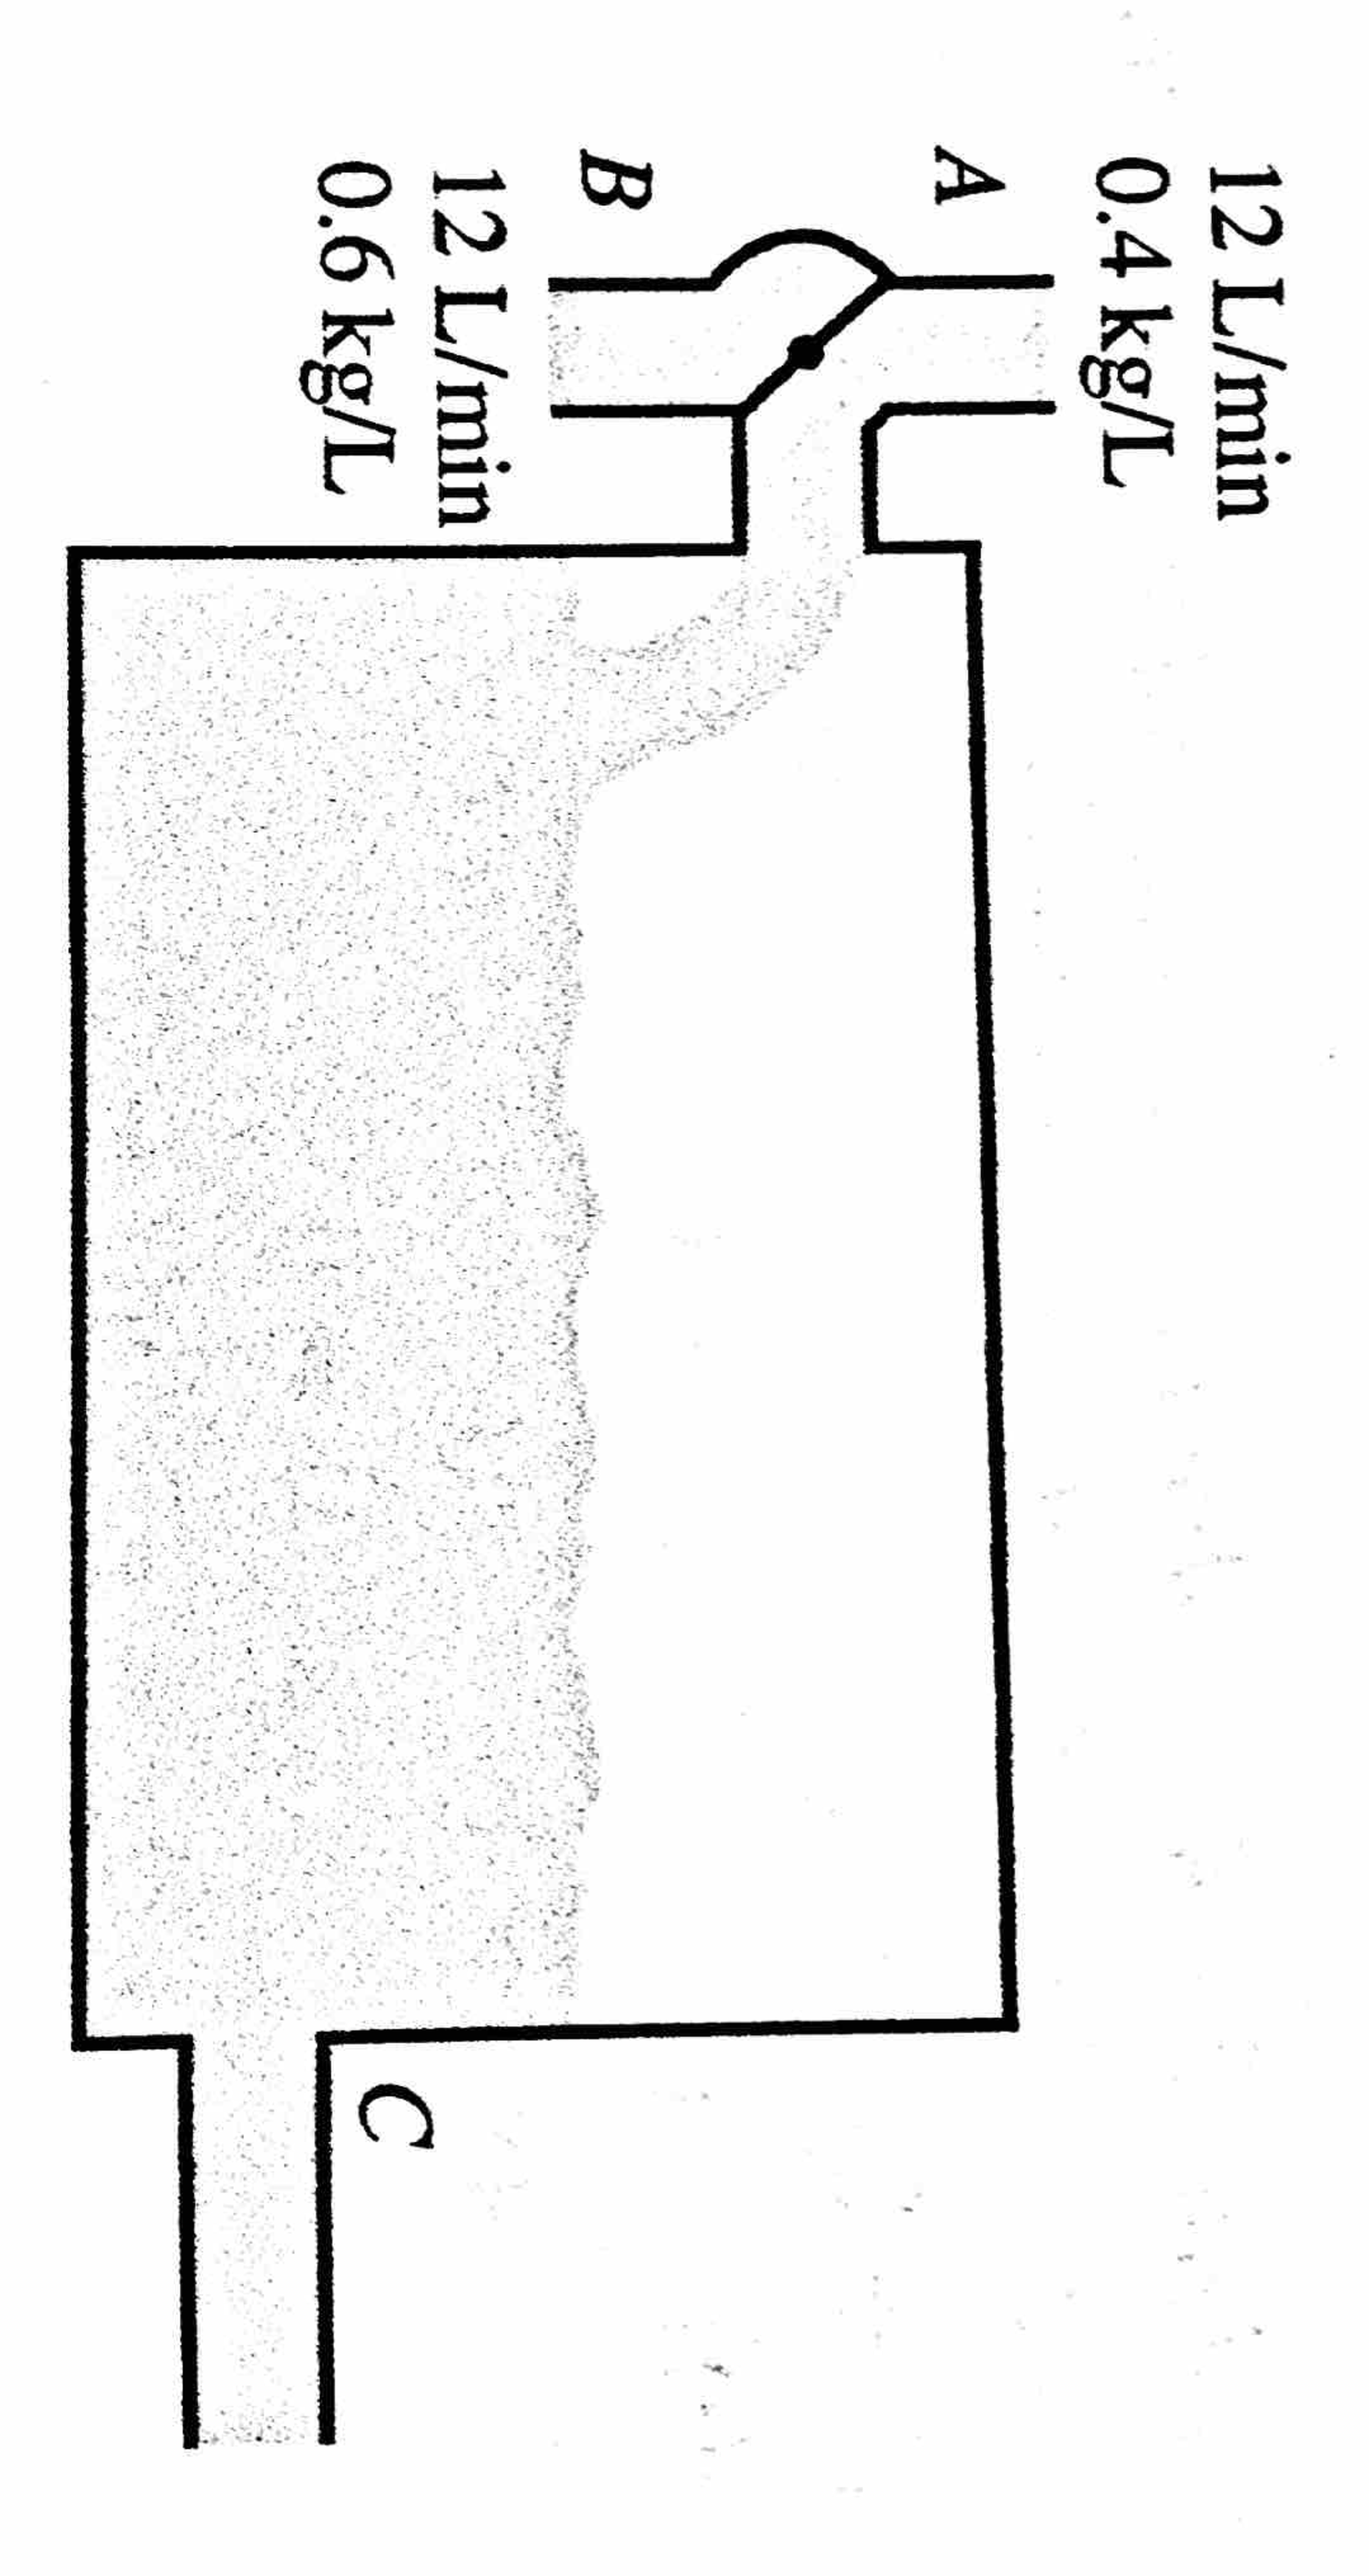
\includegraphics[angle=90,width=0.5\textwidth]{./figs/sampleProb.pdf}
\caption{Problem \label{fig:prob}}
\end{figure}
\textbf{Solution:}\\
\begin{itemize}
\item Reformulate the problem:
 The operation of the two inkets A and B is controlled by a valve.  The volume flow rate is $\dot{V}_A=\dot{V}_B=\dot{V}_{out}$. At $t=0$, $V_0=500$ L and $c=0.2$ kg/L. During time $0<t<10$ A is open, during $10<t<\infty$ B is open. \\
 We write out the mass balance:
 \begin{align*}
 \frac{dV}{dt}=\dot{V}_{in}-\dot{V}_{out} \\
 \text{or}\\
 \frac{dm}{dt}=\dot{m}_{in}-\dot{m}_{out} \\ 
 \end{align*}
where $\dot{m}=\dot{V}c$. We define our incoming mass flow rate:
 \begin{align*}
 \dot{m}_{in}=
 \begin{cases}
 (0.4)(12) \text{ kg/min for }0<t<10\\
  (0.6)(12) \text{ kg/min for }t>10\\
 \end{cases}
\end{align*}
The outgoing mass flow rate is:
 \begin{align*}
 \dot{m}_{out}= c(t)(12) \text{ kg/min for } t>0\\
\end{align*}
In the tank, we have:
 \begin{align*}
m=c(t) V=500 c(t)
\end{align*}
where $V$ is the volume of the tank. We can sub into our ODE:
 \begin{align*}
 \frac{d [500 c(t)]}{dt}=
  \begin{cases}
 (0.4-c(t))12 \text{ kg/min for }0<t<10\\
  (0.6-c(t))12 \text{ kg/min for }t>10\\
 \end{cases}
 \end{align*}
 
 \begin{align*}
 \frac{d [ c(t)]}{dt}=
  \begin{cases}
 (0.4-c(t))0.024 \text{ kg/min for }0<t<10\\
  (0.6-c(t))0.024 \text{ kg/min for }t>10\\
 \end{cases}
 \end{align*}
\item Treatment of discontinuities:
We now need to express the ODE using Heaviside function for the forcing term:
 \begin{align*}
f(t)=0.024(0.4-c)[h(t-0)-h(t-10)] + 0.024(0.6-c)[h(t-10)]
 \end{align*}
 for $t>0$.
We can rewrite the equation as:
 \begin{align*}
f(t)&=0.024(0.4-c) - 0.024(0.4-c)[h(t-10)] + 0.024(0.6-c)[h(t-10)]\\
&=0.024(0.4-c)+0.0048h(t-10)
 \end{align*}
 our ODE becomes:
  \begin{align*}
\frac{d [ c(t)]}{dt}=0.0096-0.024c +0.0048h(t-10)
 \end{align*}
 or
  \begin{align*}
\frac{d [ c(t)]}{dt}+0.024c=0.0096 +0.0048h(t-10)
 \end{align*} 
\item LT to solve our ODE:
  \begin{align*}
\Lapl{\frac{d [ c(t)]}{dt}+0.024c}=\Lapl{0.0096 +0.0048h(t-10)}\\
\Lapl{\frac{d [ c(t)]}{dt}+0.024c}&=sC(s)-c(0)+0.024C(s)\\
% &=sC(s)-0.2+0.024C(s)
 \end{align*} 
our RHS becomes:
  \begin{align*}
\Lapl{0.0096 +0.0048h(t-10)}&=\Lapl(0.0096)+0.0048\Lapl(h(t-10))\\
&=0.0096\frac{1}{s}+0.0048\frac{e^{-10s}}{s}
 \end{align*} 
 combine together:
  \begin{align*}
sC(s)-0.2+0.024C(s)=(s+0.0024)C(s)-0.2=0.0096\frac{1}{s}+0.0048\frac{e^{-10s}}{s}
 \end{align*} 
We obtain: 
  \begin{align*}
\boxed{C(s)=0.0096\frac{1}{s(s+0.0024)}+0.0048\frac{e^{-10s}}{s(s+0.0024)}+0.2\frac{1}{s+0.0024}}
 \end{align*} 
\item Factor out some terms:
  \begin{align*}
\frac{1}{s(s+0.024)}=\left(\frac{1}{s}-\frac{1}{s+0.024}\right)\frac{1}{0.024}
 \end{align*}
We can write our equation as:
  \begin{align*}
C(s)=0.4\underbrace{\left(\frac{1}{s}-\frac{1}{s+0.024}\right)}_{}(1)+0.2\underbrace{e^{-10s}\left(\frac{1}{s}-\frac{1}{s+0.024}\right)}_{(2)}+0.2\underbrace{\frac{1}{s+0.0024}}_{(3)}
 \end{align*}
 \item Inverse LT\\
 \begin{align*}
 c(t)=\Lapl^{-1}(C(s))=\Lapl^{-1}((1))+\Lapl^{-1}((2))+\Lapl^{-1}((3))
 \end{align*}
 We have:
 \begin{align*}
\Lapl^{-1}((1))&=0.4\left(\Lapl^{-1}[\frac{1}{s}]-\Lapl^{-1}[\frac{1}{s+0.024}]\right)\\
&=0.4\left(1-e^{-0.024t}\right)
 \end{align*}

 \begin{align*}
\Lapl^{-1}((2))&=0.2\underbrace{\Lapl^{-1}[e^{-10s}\frac{1}{s}]}_{(2a)}  -0.2\underbrace{\Lapl^{-1}[e^{-10s}\frac{1}{s+0.024}]}_{(2b)}
 \end{align*} 
 For 2a:
  \begin{align*}
\Lapl^{-1}(e^{-as}F(s))=h(t-a)f(t-a)\\
\Lapl^{-1}(e^{-10s}\frac{1}{s})=h(t-10)f(t-a)\\
 \end{align*} 
 Since $f(t)=\Lapl^{-1}(\frac{1}{s})=1$ we have: $\Lapl^{-1}(e^{-10s}\frac{1}{s})=h(t-10)$
 [continue at home]
\end{itemize}
\end{exmp}
